\documentclass[border={1.5mm 0.6mm}]{standalone}
\usepackage[T1]{fontenc}
\usepackage{newtxtext,newtxmath}
\usepackage{xcolor}
\usepackage{tikz}
\usepackage{pgfplots}
\usepackage{amsmath}
\pgfplotsset{compat=1.18}
\usetikzlibrary{arrows.meta,calc,positioning,decorations.pathreplacing,fit,backgrounds,patterns,shapes.misc,shapes.geometric}
\usepgfplotslibrary{groupplots,fillbetween}
\definecolor{ink}{HTML}{111111}
\definecolor{accent}{HTML}{A8321F}
\definecolor{steel}{HTML}{1F4A7A}
\definecolor{midgray}{HTML}{6E6E6E}
\definecolor{lightgray}{HTML}{D9D9D9}
\newcommand{\figsize}{\fontsize{8}{9.6}\selectfont}
\newcommand{\smallsize}{\fontsize{7}{8.4}\selectfont}
\AtBeginDocument{\DeclareFontShape{OML}{ntxmi}{m}{it}{<-> ntxmi}{}\frenchspacing}
\pgfplotsset{
  every axis/.append style={
    axis line style={line width=0.45pt,ink},
    tick style={line width=0.4pt,ink},
    major tick length=3pt,
    minor tick length=1.6pt,
    tick align=inside,
    xtick pos=both,
    ytick pos=both,
    minor tick num=0,
    grid=none,
    label style={font=\figsize},
    tick label style={font=\figsize},
    legend style={font=\smallsize,draw=none,fill=none,inner sep=1pt,row sep=-0.5pt},
    legend cell align=left,
    xlabel near ticks,
    ylabel near ticks,
    /pgf/number format/1000 sep={\mbox{,}},
    scaled ticks=false,
    clip marker paths=true,
  },
  x25519/.style={ink,line width=0.5pt,solid,mark=*,mark size=1.0pt,mark options={solid,fill=ink,line width=0.2pt}},
  hybrid/.style={accent,line width=0.5pt,solid,mark=square*,mark size=0.95pt,mark options={solid,fill=accent,line width=0.2pt}},
  x25519open/.style={ink,only marks,mark=*,mark size=1.25pt,mark options={solid,fill=white,line width=0.45pt}},
  hybridopen/.style={accent,only marks,mark=square*,mark size=1.15pt,mark options={solid,fill=white,line width=0.45pt}},
}
\newcommand{\panel}[1]{{\figsize(#1)}}

\begin{document}
\figsize
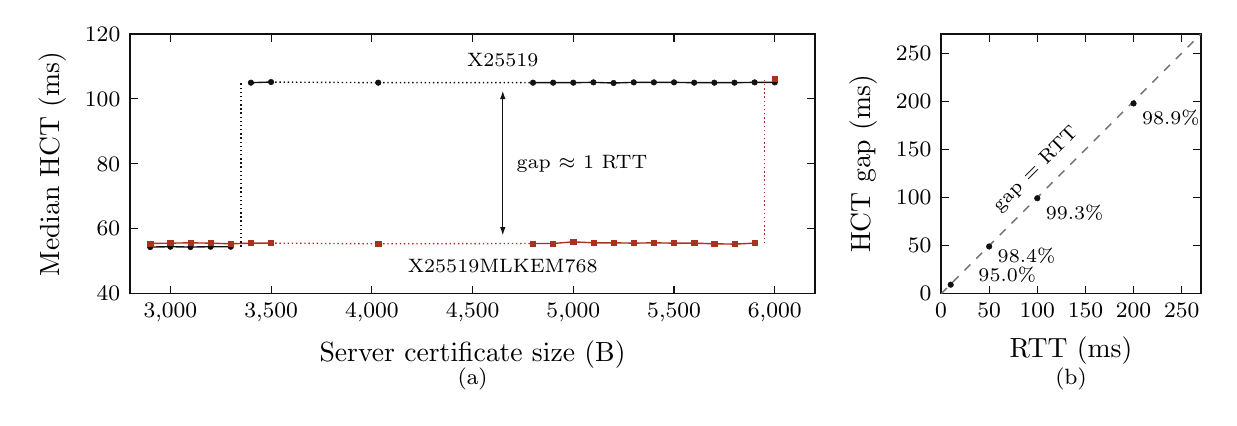
\begin{tikzpicture}
\path (-13mm,-13.2mm) rectangle (137mm,33.8mm);
\begin{axis}[name=A,at={(0,0)},anchor=south west,scale only axis,width=87mm,height=33mm,
  xmin=2800,xmax=6200,ymin=40,ymax=120,xtick={3000,3500,...,6000},ytick={40,60,...,120},
  xlabel={Server certificate size (B)},ylabel={Median HCT (ms)}]
\addplot[x25519,forget plot] coordinates {(2900,54.4) (3000,54.5) (3100,54.4) (3200,54.5) (3300,54.5)};
\addplot[x25519,forget plot] coordinates {(3400,105) (3500,105.2)};
\addplot[x25519,forget plot] coordinates {(4800,105) (4900,105) (5000,105) (5100,105.1) (5200,104.9) (5300,105.1) (5400,105.1) (5500,105.1) (5600,105) (5700,105) (5800,105) (5900,105.1) (6000,105.1)};
\addplot[x25519,only marks,forget plot] coordinates {(4032,105)};
\addplot[ink,line width=0.5pt,densely dotted,forget plot] coordinates {(3350,54.5) (3350,105)};
\addplot[ink,line width=0.5pt,densely dotted,forget plot] coordinates {(3500,105.2) (4032,105) (4800,105)};

\addplot[hybrid,forget plot] coordinates {(2900,55.5) (3000,55.6) (3100,55.7) (3200,55.6) (3300,55.4) (3400,55.6) (3500,55.6)};
\addplot[hybrid,forget plot] coordinates {(4800,55.5) (4900,55.5) (5000,56) (5100,55.7) (5200,55.7) (5300,55.6) (5400,55.7) (5500,55.6) (5600,55.6) (5700,55.4) (5800,55.3) (5900,55.6)};
\addplot[hybrid,only marks,forget plot] coordinates {(6000,106.2)};
\addplot[hybrid,only marks,forget plot] coordinates {(4032,55.4)};
\addplot[accent,line width=0.5pt,densely dotted,forget plot] coordinates {(5950,55.6) (5950,106.2)};
\addplot[accent,line width=0.5pt,densely dotted,forget plot] coordinates {(3500,55.6) (4032,55.4) (4800,55.5)};

\node[font=\smallsize,anchor=south] at (axis cs:4650,107) {X25519};
\node[font=\smallsize,anchor=north] at (axis cs:4650,53.5) {X25519MLKEM768};
\draw[{Latex[length=3pt,width=2pt]}-{Latex[length=3pt,width=2pt]},line width=0.4pt,ink] (axis cs:4650,58) -- (axis cs:4650,102.5);
\node[font=\smallsize,anchor=west] at (axis cs:4670,80) {gap $\approx$ 1 RTT};
\end{axis}
\node[anchor=north] at ($(A.south)+(0,-8.2mm)$) {\panel{a}};
\begin{axis}[name=B,at={(103mm,0)},anchor=south west,scale only axis,width=33mm,height=33mm,
  xmin=0,xmax=270,ymin=0,ymax=270,xtick={0,50,...,250},ytick={0,50,...,250},
  xlabel={RTT (ms)},ylabel={HCT gap (ms)}]
\addplot[midgray,line width=0.45pt,dashed,forget plot] coordinates {(0,0)(270,270)};
\addplot[x25519,only marks,forget plot] coordinates {(10,9.5) (50,49.2) (100,99.3) (200,197.8)};
\node[font=\smallsize,anchor=west,inner sep=1.5pt] at (axis cs:34,20) {95.0\%};
\node[font=\smallsize,anchor=north west,inner sep=1.5pt] at (axis cs:54,52.2) {98.4\%};
\node[font=\smallsize,anchor=north west,inner sep=1.5pt] at (axis cs:104,97.3) {99.3\%};
\node[font=\smallsize,anchor=north west,inner sep=1.5pt] at (axis cs:204,195.8) {98.9\%};
\node[font=\smallsize,rotate=45,anchor=south] at (axis cs:112,116) {gap $=$ RTT};
\end{axis}
\node[anchor=north] at ($(B.south)+(0,-8.2mm)$) {\panel{b}};
\pgfresetboundingbox
\path (-13mm,-13.2mm) rectangle (137mm,33.8mm);
\end{tikzpicture}
\end{document}
